\documentclass[t]{beamer}
\usetheme{Copenhagen}
\setbeamertemplate{headline}{} % remove toc from headers
\beamertemplatenavigationsymbolsempty

\usepackage{amsmath, tikz, pgfplots, tcolorbox, xcolor, array}
\pgfplotsset{compat = 1.16}

\tikzstyle{input} = [circle, text centered, radius = 1cm, draw = black]
\tikzstyle{function} = [rectangle, text centered, minimum width = 2cm, minimum height = 1cm, draw = black]

\title{Compositions of Functions}
\author{}
\date{}

\AtBeginSection[]
{
  \begin{frame}
    \frametitle{Objectives}
    \tableofcontents[currentsection]
  \end{frame}
}

\begin{document}

\begin{frame}
    \maketitle
\end{frame}

\section{Evaluate the composition of two functions at a value}

\begin{frame}{Evaluating the Composition of Two Functions}
Compositions of functions involve {\color{blue}\textbf{substituting}} one function into the variable(s) of another.	\newline\\	\pause

The composition of a function $f$ and $g$ denoted
\[ (f \circ g)(x) \]
is
\[(f \circ g)(x) = f(g(x)) \]

where we plug $g(x)$ into the variable for $f(x)$.	\newline\\	\pause

In other words, the output of $g(x)$ becomes the input of $f(x)$.
\end{frame}

\begin{frame}{Functions as Machines}
The following illustrates finding $(f \circ g)(8)$ in which \[g(x)=2x+3 \text{ and } f(x) = x^2\]:		\pause

\begin{center}
    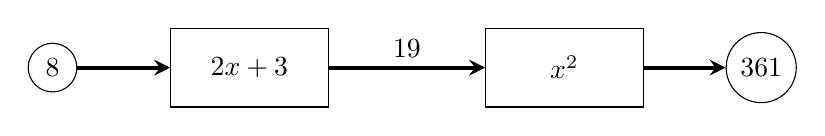
\begin{tikzpicture}[node distance = 2.5cm]
    \node (inputVal) [input] {8};
    \node (fx) [function, right of = inputVal] {$2x + 3$};
    \node (gx) [function, right of = fx, node distance = 4cm] {$x^2$};
    \node (outputVal) [input, right of = gx] {361};
    \node at (4.5,0) [anchor = south] {19};
    
    \draw [->, >=stealth, line width = 1.5] (inputVal) -- (fx);
    \draw [->, >=stealth, line width = 1.5] (fx) -- (gx);
    \draw [->, >=stealth, line width = 1.5] (gx) -- (outputVal);
    \end{tikzpicture}
\end{center}	\pause
\begin{enumerate}
\item<+-> Evaluate $g(8)$ to get $2(8)+3$, or 19. \newline\\
\item<+-> Evaluate $f(19)$ to get $19^2$, or 361.
\end{enumerate}
\end{frame}

\begin{frame}{Example 1}
Find each of the following if $f(x) = 3x-4$ and $g(x) = x^2 + 6$	\newline\\
(a) \quad $(f \circ g)(2)$
\begin{align*}
\onslide<2->{(f \circ g)(2) &= f({\color{red}g(2)})} \\[6pt]
\onslide<3->{g(2) &= 2^2 + 6} \\[6pt]
\onslide<4->{g(2) &= \color{red}10} \\[6pt]
\onslide<5->{f({\color{red}10}) &= 3({\color{red}10})-4} \\[6pt]
\onslide<6->{&= 26}
\end{align*}
\end{frame}

\begin{frame}{Example 1 \quad $f(x)=3x-4 \quad g(x)=x^2+6$}
(b) \quad $(g \circ f)(2)$
\begin{align*}
\onslide<2->{(g \circ f)(2) &= g({\color{blue}f(2)})} \\[6pt]
\onslide<3->{f(2) &= 3(2)-4} \\[6pt]
\onslide<4->{f(2) &= \color{blue}2} \\[6pt]
\onslide<5->{g({\color{blue}2}) &= {\color{blue}2}^2+6} \\[6pt]
\onslide<6->{&= 10}
\end{align*}
\end{frame}

\begin{frame}{Example 1 \quad $f(x)=3x-4 \quad g(x)=x^2+6$}
(c) \quad $(f \circ f)(1)$
\begin{align*}
\onslide<2->{(f \circ f)(1) &= f({\color{blue}f(1)})} \\[6pt]
\onslide<3->{f(1) &= 3(1)-4} \\[6pt]
\onslide<4->{f(1) &= \color{blue}-1} \\[6pt]
\onslide<5->{f({\color{blue}-1}) &= 3({\color{blue}-1})-4} \\[6pt]
\onslide<6->{&= -7}
\end{align*}
\end{frame}


\section{Write the composition of two functions}


\begin{frame}{Writing the Composition of Two Functions}
We can even substitute an entire function into another and simplify.	\newline\\	\pause

Using $\color{red}g(x)=2x+3$ and $\color{blue}f(x)=x^2$, the composition $(f \circ g)(x)$ becomes
\begin{align*}
\onslide<3->{({\color{blue}f} \circ {\color{red}g})(x) &= {\color{blue}f}({\color{red}2x+3})} \\[6pt]
\onslide<4->{&=({\color{red}2x+3})^2} \\[6pt]
\onslide<5->{&=(2x+3)(2x+3)} \\[6pt]
\onslide<6->{&=4x^2 + 12x + 9}
\end{align*}
\end{frame}

\begin{frame}{Example 2}
Find each of the following if $f(x) = 3x-4$ and $g(x)=x^2+6$	\newline\\
(a) \quad $(f \circ g)(x)$
\begin{align*}
\onslide<2->{(f \circ g)(x) &= {\color{red}f({\color{blue}g(x)})}} \\[6pt]
\onslide<3->{&= {\color{red}3({\color{blue}x^2+6})-4}} \\[6pt]
\onslide<4->{&= 3x^2 + 18 \color{red}- 4} \\[6pt]
\onslide<5->{&= 3x^2 + 14}
\end{align*}
\end{frame}

\begin{frame}{Example 2 \quad $f(x) = 3x-4$ and $g(x)=x^2+6$}
(b) \quad $(g \circ f)(x)$
\begin{align*}
\onslide<2->{(g \circ f)(x) &= {\color{blue}g({\color{red}f(x)})}} \\[6pt]
\onslide<3->{&= {\color{blue}({\color{red}3x-4})^2+6}} \\[6pt]
\onslide<4->{&= 9x^2-12x-12x+16 \color{blue} +6} \\[6pt]
\onslide<5->{&= 9x^2- 24x + 22}
\end{align*}
\end{frame}

\begin{frame}{Example 2 \quad $f(x) = 3x-4$ and $g(x)=x^2+6$}
(c) \quad $(f \circ f)(x)$
\begin{align*}
\onslide<2->{(f \circ f)(x) &= \color{red}f({\color{black}f(x)})} \\[6pt]
\onslide<3->{&= {\color{red}3({\color{black}3x-4})-4}} \\[6pt]
\onslide<4->{&=  9x-12\color{red} -4} \\[6pt]
\onslide<5->{&= 9x-16}
\end{align*}
\end{frame}

\begin{frame}{Evaluating the Composition of Functions}
In the previous video, we looked at things like 
\[(f \circ g)(2) \] 

We could also evaluate our answer for $(f \circ g)(x)$ at $x = 2$.
\end{frame}

\end{document}
